\begin{figure*}[t]
    \centering
    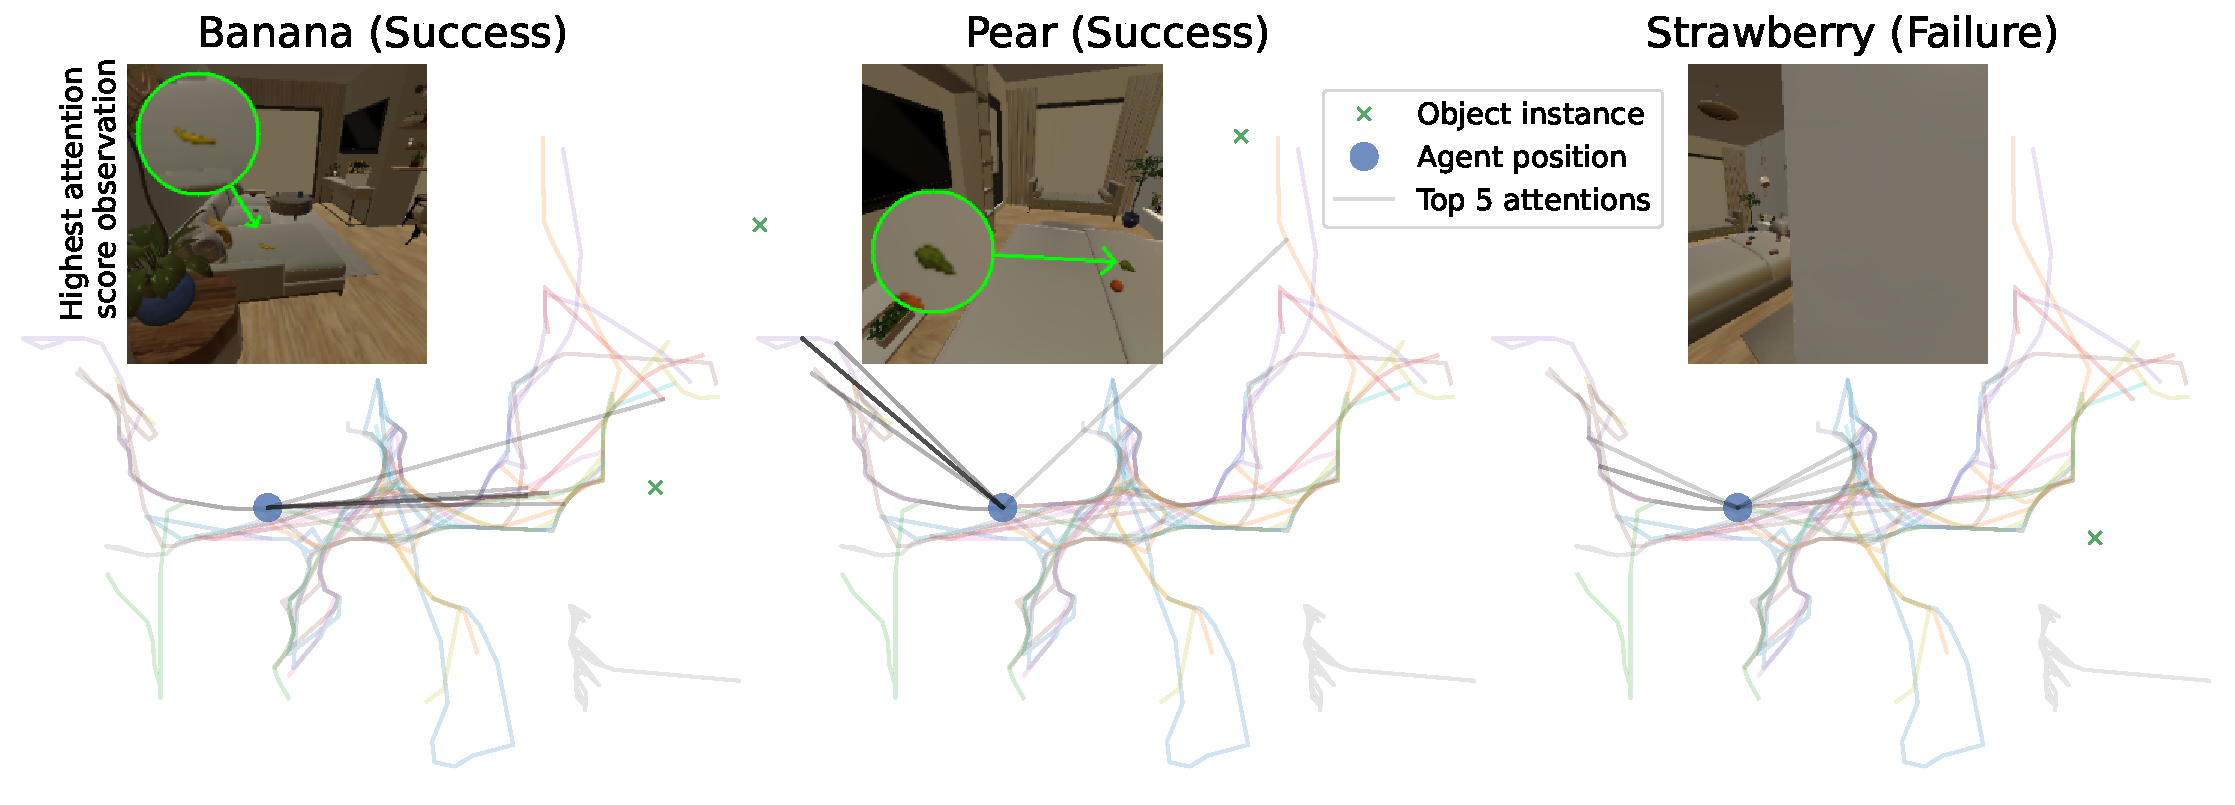
\includegraphics[width=\textwidth]{figures/results/trajectory_object_attn_3s_v5.pdf}
    \vspace{-15pt}
    \caption{Visualization of an inter-episode attention head, see \Cref{sec:app-what-agent-see}. The colored curves are the trajectories of previous episodes. The blue circle is the agent's position. The green Xs are the instances of the target object type. The black lines represent the agent's attention when the target is the object type mentioned above the image. The lines connect the agent with the point in history that it attends to, the opacity of the line represents the attention score. The overlaid image is visual observation with the highest attention score.}
    \label{fig:trajectory_object_attn_4s}
    \vspace{-15pt}
\end{figure*}

\begin{figure*}[t]
    \centering
    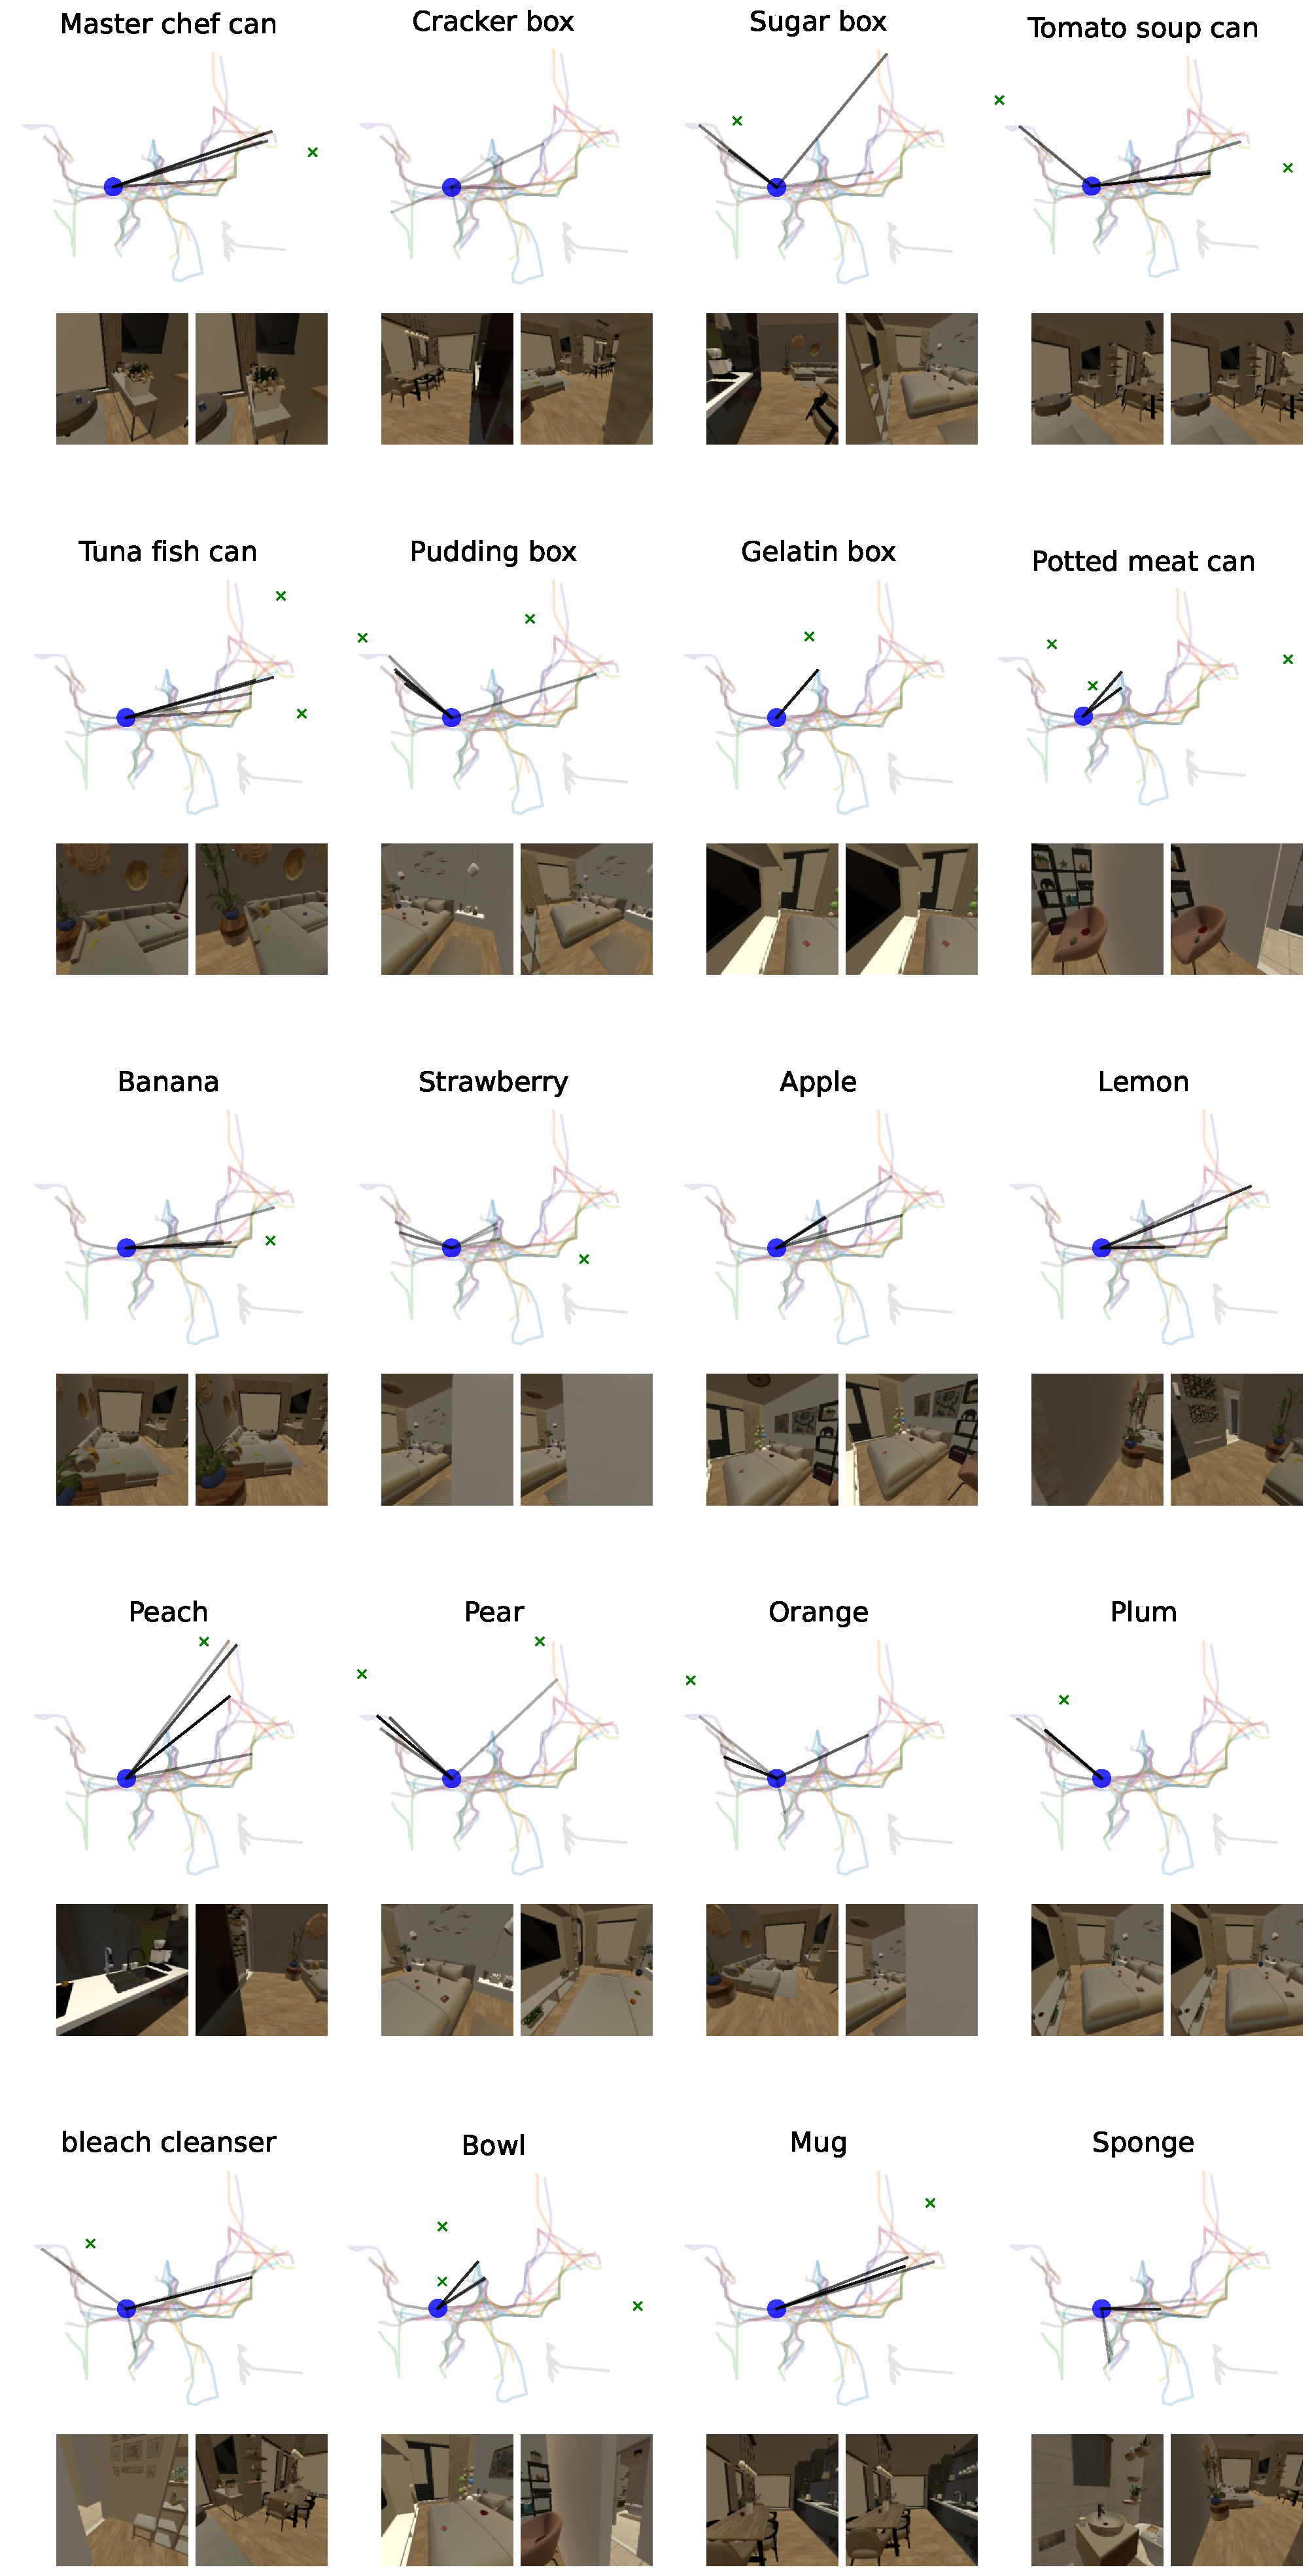
\includegraphics[width=\textwidth,height=0.9\textheight,keepaspectratio]{figures/results/trajectory_object_attn_all.pdf}
    \caption{Attention scores of the object detection head described in \Cref{sec:app-what-agent-see}. The colored curves are the trajectories of previous episodes. The blue circle is the agent's position. The black lines represent the agent's attention when the target is the type in above the image. The lines connect the agent with the point in history that it attends to, the opacity of the line represents the attention score. The two images with highest attention score are shown in the 3rd row.}
    \label{fig:app_trajectory_object_attn_4s}
\end{figure*}
